\subsection{Matos obligatoire}

\begin{frame}{Équipement obligatoire de plongée}
{Article A322-80 et A322-81 du Code du Sport}
\begin{block}<only@-6>{Article A322-80}
\only<1-3>{Chaque bouteille ou ensemble de bouteilles d'un même gaz respirable est muni
d'un \only<1>{manomètre}\only<2->{\Emph{manomètre}} ou d'un système équivalent permettant d'indiquer la pression au
cours de la plongée.  En milieu naturel, chaque plongeur équipé d'un appareil à
circuit ouvert est muni d'\only<-2>{un système gonflable au moyen de gaz comprimé lui
permettant de regagner la surface et de s'y maintenir.}\only<3>{\Emph{un système gonflable au moyen de gaz comprimé lui
permettant de regagner la surface et de s'y maintenir.}}}
\only<4>{%
En milieu naturel, chaque plongeur encadré au-delà de \numprint{20}~mètres et
chaque plongeur en autonomie est muni:
\begin{itemize}
\item D'un équipement de plongée permettant d'alimenter en gaz respirable un
  équipier sans partage d'embout;
\item D'équipements permettant de contrôler les caractéristiques personnelles
de sa plongée et de sa remontée.
\end{itemize}
}\only<5>{%
En milieu naturel, la personne encadrant la palanquée est munie:
\begin{itemize}
\item D'un équipement de plongée avec deux sorties indépendantes et deux
  détendeurs complets;
\item D'un système gonflable au moyen de gaz comprimé lui permettant de
  regagner la surface et de s'y maintenir;
\item D'équipements permettant de contrôler les caractéristiques de la plongée
  et de la remontée de sa palanquée.
\end{itemize}
}\only<6>{%
En milieu naturel, chaque palanquée dispose d'un parachute de palier.
}
\end{block}
\begin{itemize}[<only@7>]
\item Manomètre;
\item gilet;
\item octopus;
\item ordinateur ou tables/profondimètre/chronomètre;
\item parachute.
\end{itemize}
\begin{block}<only@8->{Article A322-81}
Les matériels subaquatiques et équipements nautiques utilisés par les plongeurs
sont \only<8>{régulièrement vérifiés}\only<9>{\emph{régulièrement vérifiés}} et
\only<8>{correctement entretenus}\only<9>{\emph{correctement entretenus}}.

Les tubas et les détendeurs mis à disposition des plongeurs par les
établissements sont désinfectés avant chaque plongée en cas de changement
d'utilisateur.
\end{block}
\end{frame}

\subsection{Comment que ça marche?}
\subsubsection{Bouteille}

\begin{frame}{Obligations légales}
\begin{block}<only@1>{\chref{https://www.legifrance.gouv.fr/loda/article_lc/LEGIARTI000036131133}{Arrêté du 20 novembre 2017}}
\small
\begin{itemize}
\item deux ans pour les bouteilles pour appareils respiratoires utilisées pour la
  plongée subaquatique ainsi que pour les récipients mobiles en matériaux
  autres que métalliques;
\item six ans pour les bouteilles de plongée dont l'inspection périodique a été
  effectuée au moins annuellement ou avant leur utilisation quand la visite a
  été réalisée depuis plus d'un an, dans les conditions définies par la dernière
  version du cahier des charges relatif à l'inspection périodique des bouteilles
  métalliques utilisées pour la plongée subaquatique visé en annexe 1 du présent
  arrêté ministériel;
\end{itemize}
\end{block}%
\begin{block}<only@1>{Arrêté du 09 avril 2020}
\chref{https://ffessm.fr/actualites/suivi-des-equipements-sous-pression}{Commenté}
notamment sur le site de FFESSM. Ne change en pratique rien.
\end{block}%
\begin{block}<only@2>{Au final}
\begin{itemize}
\item T.I.V. tous les ans;
\item requalification:
  \begin{itemize}
    \item tous les deux ans sous régime général;
    \item tous les six ans sous régime spécial.
  \end{itemize}
\end{itemize}
\end{block}
\end{frame}

\begin{frame}{Entretien/usage/\dots}
\only<-3>{\begin{itemize}
\item<1-> Éviter la corrosion:
  \begin{itemize}
    \item robinet fermé! Si ouvert l'humidité entre;
    \item ne pas vider brutalement! Choc thermique\footnote{Cela provoque une
        détente adiabatique (pour les deux physiciens du fond).} qui va refroidir
        et faire condenser l'humidité contenue dans le bloc.
  \end{itemize}
\item<2-> Éviter de l'abîmer:
  \begin{itemize}
    \item éviter les chocs, utiliser un filet;
    \item se conserve debout: le peu d'eau corrodra
      le fond, plus épais;
    \item ne pas laisser à la chaleur (sous cagnard, coffre
      voiture).
  \end{itemize}
\item<3> Utilisation sécurisée et correcte:
  \begin{itemize}
    \item Bloc gréé, bloc allongé!
    \item Ne sert pas le détendeur comme une brute! Doucement sur les joints.
    \item Sécher le robinet en lachant un peu d'air en fin de plongée.
  \end{itemize}
\end{itemize}}%
\only<4->{Le cas du transport.
\begin{itemize}[<+(3)->]
\item Ne bouge/roule pas;
\item protège les robinets;
\item le sens de la bouteille\dots
\end{itemize}}
\end{frame}

\begin{frame}{Le bloc}
\centering
%bouteille complete
\begin{tikzpicture}
\node<1> (bloc) at (0,0) {\includegraphics[angle=-90,width=3cm]{bloc_1}};%
\path<1>[use as bounding box] (bloc.north east) rectangle (bloc.south west);
\draw<1>[thick,blue] (bloc.145) -- (bloc.35);
\node<1>[right] at (bloc.50) {Robinet(s)};
\node<1>[left,align=right] at (bloc.180) {Corps\\acier, aluminium};
%robinets
\node<2-> (rob) at (0,0) {\includegraphics[angle=-90,width=0.5\textwidth,viewport=300 120 620 750,clip]{bloc_1}};%
\path<2->[use as bounding box] (rob.north east) rectangle (rob.south west);
\node<2->[circle,minimum height=9mm,pin={[pin edge={thick,stealth-},pin distance=2cm]45:Étrier}] at (0.95,0.05) {};
\node<2->[circle,minimum height=9mm,pin={[pin edge={thick,stealth-}]above:Deutsches Institut für Normung (D.I.N.)}] at (-1.3,0.9) {};
\node<2->[circle,inner sep=0pt,minimum height=3mm,pin={[visible on=<3->,pin edge={visible on=<3->,red,Circle-},pin distance=2cm,name=joint]right:Joint}] at (0.95,0.05) {};
\draw<2->[visible on=<3->,red,Circle-,very thin] (0.95,0.05) -- ++(-30:1.2) -- ++(1.11,0) node[right,black] (ope) {Opercule};
\node<4->[fit=(joint) (ope),draw,red,circle,inner sep=1pt,pin=below:Savoir les changer] {};
\end{tikzpicture}
\end{frame}

\begin{frame}{Papiers!}
\centering
\begin{tikzpicture}[every pin edge/.style={red}]
%% bouteille
\node<-3> (bloc) at (0,0) {\includegraphics[width=\frameheight-8pt,angle=-90]{bloc_2}};
\node<4-8> (bloc) at (0,0) {\includegraphics[width=\frameheight-8pt,angle=-90]{bloc_3}};
\node<9-12> (bloc) at (0,0) {\includegraphics[width=\frameheight-8pt,angle=-90]{bloc_4}};
\node<13-> (bloc) at (0,0) {\includegraphics[width=\frameheight-8pt,angle=-90,viewport=200 80 1900 845,clip]{bloc_1}};
\path[use as bounding box] (bloc.north east) rectangle (bloc.south west);
\node<2-3>[draw,red,rounded corners=5pt,pin={[pin distance=1cm]left:Mélange gazeux},minimum width=2cm,minimum height=5mm] at (0,0.05) {};
\node<3>[draw,red,pin={[pin distance=8mm]45:Pas de vis},circle] at (0.9,0.5) {};
\node<4-8>[draw,red,pin={[pin distance=1.2cm]130:Pas de vis},circle] at (-0.7,0.9) {};
\node<5-8>[draw,red,pin={[pin distance=1.2cm]200:Masse du bloc},rounded corners=2pt,minimum width=8mm,minimum height=2mm] (masse) at (-0.28,0.45) {};
\node<6-8>[anchor=west,draw,red,pin={[pin distance=1.3cm,align=left]-40:Volume interne\\du bloc},rounded corners=2pt,minimum width=5.5mm,minimum height=2mm] (vol) at (masse.east) {};
\node<7-8>[draw,red,pin={[pin distance=1cm]20:Pression de service},rounded corners=2pt,minimum width=5mm,minimum height=10pt,above right] at ([yshift=-2pt]vol.east) {};
\draw<8>[draw,red,rounded corners=2pt] (-0.55,0.2) rectangle ++(1,-1);
\node<9-12>[draw,red,pin={[pin distance=1.2cm]180:Pression de service},rounded corners=2pt,minimum width=6mm,minimum height=3mm] (ps) at (-0.76,0.5) {};
\node<10-12>[draw,red,pin={[pin distance=2cm, align=right]220:Température\\de référence},rounded corners=2pt,minimum width=6.5mm,minimum height=2mm,right] (at) at ([yshift=2pt]ps.south east) {};
\node<11-12>[draw,red,pin={[pin distance=1cm]0:Pression de test},rounded corners=2pt,minimum width=8mm,minimum height=3mm,right] (pt) at (at.east) {};
\node<12>[draw,red,pin={[pin distance=1.6cm]140:Fabricant},rounded corners=2pt,minimum width=5mm,minimum height=3mm,right] at (-0.67,0.85) {};
\node<13->[draw,red,pin={[pin distance=1.6cm,align=right]140:Température\\de service},rounded corners=2pt,minimum width=7mm,minimum height=3mm] at (-0.7,0.6) {};
\node<14->[draw,red,pin={[pin distance=1.5cm,align=right]10:Épaisseur},rounded corners=2pt,minimum width=5mm,minimum height=3mm] at (0.4,1) {};
\node<15->[draw,red,pin={[pin distance=1.6cm,align=right]0:Date de [ré]épreuve},rounded corners=2pt,minimum width=6mm,minimum height=3mm] (dr) at (0.15,0.55) {};
\draw<16>[red] ([xshift=-3pt]dr.west) circle(2pt);
\draw<16>[red,path picture={\node at (path picture bounding box.center) {\includegraphics[angle=-90,viewport=900 380 950 430,clip]{bloc_1}};}] 
  (-3,-1) circle(15pt);
\path<16> ([xshift=-3pt,yshift=2pt]dr.west) coordinate(su) ([xshift=-3pt,yshift=-2pt]dr.west)coordinate(sd)
  (-3,-1) +(100:15pt) coordinate (bu) +(-67:15pt) coordinate (bd);
\draw<16>[red] (su) -- (bu) (sd) -- (bd);
\end{tikzpicture}
\end{frame}

\subsubsection{Gilet}

\begin{frame}{Présentation}
{Système de Sécurité Gonflable (SSG)}
Trois types:
\begin{itemize}[<+->]
\item enveloppant: \textcolor{green!60!black}{confortable, flotte à la
  verticale}, \textcolor{red!50!black}{taille non négociable};
\item dorsal: \textcolor{green!60!black}{mouvements libres, gros volume},
  \textcolor{red!50!black}{flotte sur le ventre en surface};
\item réglable: plus ou moins un enveloppant réglable.
\end{itemize}
\end{frame}

\begin{frame}{Détails}
\centering
\begin{tikzpicture}[every pin edge/.append style={thick},pin lines/.style={help lines,thick}]% Gilet »
\useasboundingbox (-5.2,-3.8) rectangle (5.2,3.8);
\node<-4,6->[left=1mm]  at (0,0) {\includegraphics[width=5cm]{gilet_recto}};
\node<-4,6->[right=1mm] at (0,0) {\includegraphics[width=5cm]{gilet_verso}};
\path<5>[path picture={\node at (path picture bounding box.center) {\includegraphics[width=6cm,viewport=600 400 900 800,clip]{gilet_recto}};}] (0,0) circle(3cm);

%%% sangles
\begin{scope}[gilet,transparency group]
\fill<2> (-4,-0.1) -- (-3.1,-1.3) -- (-2.5,-1.1) -- (-1.9,-1.6) -- (-2.75,-1.8) -- (-2.9,-2.05) -- (-3.2,-2.2) -- (-3.5,-2.2) -- (-4.3,-1) -- cycle;
\fill<2>[rotate around={-10:(-2.3,-2.3)}] (-2.3,-2.3) rectangle (-2.75,-1.5);
\fill<2> (-3.3,-2.7) rectangle (-3.95,-2.35);
\draw<2>[line width=1mm] (-3.6,-2) -- (-3.75,-2.4);
\fill<2>[rotate around={20:(-2,0.2)}]   (-2,0.2)   rectangle (-1.8,1);
\fill<2>[rotate around={10:(-3.1,0.5)}] (-3.1,0.5) rectangle (-2.9,0.9);
\fill<2>[rotate around={-10:(-1.9,0.5)}](-1.9,0.5) rectangle (-1.6,1.1);
\fill<2>[rotate around={-10:(-3.9,0.5)}](-3.9,0.5) rectangle (-3.6,1.1);
\fill<2> (1.75,0.02) -- (1.25,-0.3) -- (1.5,-0.75) -- (2.25,-0.5) -- (2.6,-0.3) -- (2.6,0.15) -- (1.9,-0.2) -- cycle;
\end{scope}
\node<2> (vent) at (-3,-3.5) {Sangles ventrales};
\node<2> (pect) at (0.5,3)   {Sangle pectorale};
\node<2> (lat)  at (-3,3)    {Sangles latérales};
\node<2>[pin={[pin distance=2cm]-70:Sangle bloc}] at (1.75,-0.6) {};
\draw<2>[pin lines] (-3.2,-2.25) -- (vent);
\draw<2>[pin lines] (-3.5,-2.8) -- (vent);
\draw<2>[pin lines] (-2.5,-2.4) -- (vent);
\draw<2>[pin lines] (-2,0.5) -- (pect);
\draw<2>[pin lines] (-3,0.7) -- (pect);
\draw<2>[pin lines] (-1.7,0.8) -- (lat);
\draw<2>[pin lines] (-3.7,0.8) -- (lat);
\node<2>[font=\Large,above] at (0,-3.8) {Sangles};

%%% purges rapide
\begin{scope}[gilet,transparency group]
%haute
\fill<3>[rotate around={20:(-3.5,2.45)}] (-3.5,2.45) circle(6pt and 1.5pt);
\fill<3> (3.45,2.05) circle(5pt and 6pt);
\draw<3> (3.45,2.1) -- ++(80:3mm);
\draw<3> (-3.48,2.52) -- (-3.27,2.18) -- (-3.3,1.5) -- (-3.25,1);
\fill<3> (-3.25,0.82) circle(3pt and 6pt);
%basse
\fill<3> (3.85,-1.6) circle(6pt and 8pt);
\draw<3> (3.85,-1.6) -- (3.9,-2.1) -- (4.13,-2.1) -- (4.27,-2.18);
\fill<3>[rotate around={-40:(4.4,-2.25)}] (4.4,-2.25) circle(6pt and 4pt);
%fenstop
\fill<3>[rotate around={-15:(-1.65,2.45)}] (-1.65,2.45) circle(7pt and 4pt);
\fill<3> (2,2) circle(7pt);
\end{scope}
\node<3>[pin={-120:Purge basse}] at (3.85,-1.6) {\rule{0pt}{8pt}\rule{6pt}{0pt}};
\node<3> (fs) at (0,2.5) {Fenstop};
\node<3> (ph) at (0,3.5) {Purge haute};
\draw<3>[pin lines,shorten >=7pt] (ph) -- (-3.5,2.45);
\draw<3>[pin lines,shorten >=7pt] (ph) -- (3.45,2.05);
\draw<3>[pin lines,shorten >=6pt] (fs) -- (-1.65,2.45);
\draw<3>[pin lines,shorten >=8pt] (fs) -- (2,2);
\node<3>[font=\Large,above] at (0,-3.8) {Purges rapides};

%%% direct system
\draw<4>[gilet] (-1.25,0.05) circle(0.7);
\node<5> (ds) at (-3.5,2) {Direct system};
\node<5>[pin=-90:Purge lente] at (-0.5,-2.3) {};
\node<5>[pin={[pin distance=7mm]200:Gonflage buccal}] at (-1.5,-1.5) {};
\draw<5>[pin lines] (-0.75,-0.25) -- (ds)
                     (1.5,0.8) -- (ds);
\node<4>[font=\Large,above] at (0,-3.8) {Direct system};
%%% anneaux
\fill<6>[gilet] (-4.75,-1.25) circle(5pt);
\fill<6>[gilet] (-3.6,1.1) circle(6pt);
\fill<6>[gilet] (-2.25,0.2) circle(5pt);
\node<6>[font=\Large,above] at (0,-3.8) {Anneaux};

%%% poches
\fill<7>[gilet] (-1,-0.25) circle(15pt and 35pt);
\fill<7>[gilet,rotate around={-10:(-4.5,0.2)}] (-4.5,0.2) circle(10pt and 30pt);
\node<7>[font=\Large,above] at (0,-3.8) {Poches};

%%% poches à plombs
\fill<8>[gilet,rotate around={-15:(-4.6,-0.8)}]  (-4.6,-0.8)  circle(5pt and 10pt);
\fill<8>[gilet,rotate around={-35:(-1.65,-1.25)}] (-1.65,-1.25) circle(7pt and 10pt);
\fill<8>[gilet] (2,0) circle(10pt);
\fill<8>[gilet] (3.1,-0.1) circle(12pt and 14pt);
\node<8>[font=\Large,above] at (0,-3.8) {Poches à plombs};

\end{tikzpicture}% «
\end{frame}

\begin{frame}{Entretien}
\begin{block}<only@1>{Précautions}
\begin{itemize}
\item Fin de plongée: vide l'eau contenue dans le gilet. 
  Gonfler le gilet puis utiliser la purge basse pour le vider. 
\item Rincer le gilet à l'eau douce à après chaque utilisation. 
\item Le stocker légèrement gonflé. 
\item Éviter de le stocker en plein soleil. 
\item Lorsque l'on a terminé une série de plongées en milieu naturel rincer
  l'intérieur du gilet: le remplir par la purge haute ou lente d'eau douce,
  le purger, remonter la purge rapide si utilisée.
\end{itemize}
\end{block}
\begin{block}<only@2>{Pannes}
\begin{itemize}
\item Fuite au niveau des purges rapides: éventuellement mettre un peu de
  graisse silicone sur la partie en plastique dur (siège du joint).
\item Fuite au niveau du raccord de branchement du direct système: remplacer
  le flexible du direct système. 
\item Le S.S.G.\footnote{Système de Sécurité Gonflable} se gonfle tout seul:
  réviser ou changer le direct système. 
\end{itemize}
\end{block}
\end{frame}

\subsubsection{Détendeur}

\begin{frame}{Types, caractéristiques\dots}
\centering
\begin{itemize}
\item D.I.N. ou étrier;\tikz[remember picture]\coordinate (de);
\item à piston ou à membrane;\tikz[remember picture]\coordinate (pm);
\item non compensé, com\tikz[remember picture]\coordinate(c);pensé, sur-compensé,\dots
\end{itemize}
\begin{tikzpicture}[overlay,remember picture,every path/.append style={thick,blue,-stealth}]
\node<2>[black] (pre) at ([xshift=-2cm,yshift=-3cm]current page.north east) {Premier étage};
\node<2>[black] (deu) at ([xshift=-3cm,yshift=3cm]current page.south) {Premier et/ou deuxième étage};
\draw<2> (pre) -- ([yshift=0.5ex]de);
\draw<2> (pre) -- ([yshift=0.5ex]pm);
\draw<2>[shorten >=3pt] (deu) -- (c);
\end{tikzpicture}
\end{frame}


\begin{frame}{Présentation}
\centering
\begin{tikzpicture}[/tikz/ampersand replacement=\&]
\path[use as bounding box] (-3.53,-3.55) rectangle (7.11,4.1);
\node (fig) at (0,0) {\includegraphics[height=7cm]{detenteur_monte}};
%HP
\draw<2->[-stealth,blue,cover on=<5>] (-2,3.2) -- ++(0.5,0) node[pos=0.5,above] (ph) {$P_\text{H}$};
\node<2->[left,align=left,font=\footnotesize,blue!70!black,cover on=<5>] at (ph.west) {\numprint[bars]{200}\\\numprint[bars]{250}\\\numprint[bars]{300}};
%PI
\draw<3->[-stealth,cyan,cover on=<5>] (-0.5,3) .. controls +(0.2,0) and +(-0.3,0.5) .. (0.5,2) node[above,pos=0.5] {$P_\text{I}$};
\fill<3->[white,opacity=0.8] (0,0.875) rectangle ++(1.1,1.1);
\node<3->[right,font=\footnotesize,cyan!70!black,align=left,cover on=<5>] at (-0.3,1.4) {\numprint{8} à \numprint[bars]{10}\\au-dessus de $P_\text{A}$\\(max \numprint{5} à \numprint{15})};
\node<5->[right,align=left] (et1c) at (1,3.3) {1\up{er} étage: passage de la\\\textcolor{blue}{pression haute} à la\\\textcolor{cyan}{pression intermédiaire}};
\node<5->[ellipse,draw,red,thick] (et1p) at (-1.05,2.95) {\rule{0pt}{14pt}\rule{7pt}{0pt}};
\draw<5->[-stealth,red,thick,rounded corners=5pt] (et1p) |- ([yshift=-10pt]et1c.north west);
%PA
\draw<4->[-stealth,cyan!50,cover on=<5>] (2.5,0.5) -- ++(-1,0) node[above, pos=0.4] (pa) {$P_\text{A}$};
\matrix<4->[above right,cyan!50!white!90!black,cover on=<5>] at (pa.south east) {
    \node[font=\footnotesize,below right] {\numprint[m]{10}}; \& \node[font=\footnotesize,below right] {\numprint[bar]{2}}; \\
    \node[font=\footnotesize,below right] {\numprint[m]{20}}; \& \node[font=\footnotesize,below right] {\numprint[bar]{3}}; \\
    \node[font=\footnotesize,below right] {\numprint[m]{30}}; \& \node[font=\footnotesize,below right] {\numprint[bar]{4}}; \\
    \node[font=\footnotesize,below right] {\dots}; \\
};
\node<5>[below right,align=left] (et2c) at (3,-1) {2\up{ème} étage: passage de\\la \textcolor{cyan}{pression intermédiaire}\\à la \textcolor{cyan!50}{pression ambiante}};
\node<5>[draw,red,circle,thick] (et2p) at (2.2,-0.1) {\rule{0pt}{30pt}};
\draw<5>[-stealth,red,thick,rounded corners=5pt] (et2p) -| (et2c);
\end{tikzpicture}
\end{frame}

\begin{frame}{Le premier étage}
\centering%
\begin{tikzpicture}% »
\path[use as bounding box] ($(-5,6)+(0,1.5mm)$) rectangle ($(5,0)-(0,1.5mm)$);
%contour
\draw[coque] (-2,6) rectangle (2,0);
\draw[coque] (-2,4) -- (-1.5mm,4) (1.5mm,4) -- (2,4);

%hp
\begin{scope}[cover on=<3->,transparency group]
\fill[rhp] ($(-2,6)+(1.5mm,-1.5mm)$) rectangle ($(-0.5mm,4)+(0,1.5mm)$)
           ($(0.5mm,6)-(0,1.5mm)$)   rectangle ($(2,4)-(1.5mm,-1.5mm)$);
\node at (1,5) {$P_\text{H}$};
\draw[ouverture=rhp] ($(-2,5.5)-(1.5mm,0)$) -- ++( 3mm,0)
                     ($( 2,5  )+(1.5mm,0)$) -- ++(-3mm,0);
\draw[stealth-] (-2,5.5) -- ++(-4mm,0) node[left]{Bloc};
\draw[-stealth] ( 2,5  ) -- ++( 4mm,0) node[right]{Manomètre};
\end{scope}
\begin{scope}[visible on=<2>]
\draw[annot] (-1,4.5) -- ++(-2,0) node[left,align=right,black]{Chambre\\haute pression};
\fill[blue] (-1,4.5) circle(1pt);
\end{scope}

%eau
\begin{scope}[cover on={<2,4->},transparency group]
\fill[eau] ($(-2,4)+(1.5mm,-1.5mm) + (-0.1pt,0)$) rectangle ($(-1.5mm,2)+(0,1mm)$)
           ($(1.5mm,4)-(0,1.5mm) + (0,0)$) rectangle ($(2,2)-(1.5mm - 0.1pt,-1mm)$);
\draw[ouverture=eau] ($(-2,3.5)-(1.5mm,0)$) -- ++( 3mm,0)
                     ($(-2,3  )-(1.5mm,0)$) -- ++( 3mm,0)
                     ($(-2,2.5)-(1.5mm,0)$) -- ++( 3mm,0)
                     ($( 2,3.5)+(1.5mm,0)$) -- ++(-3mm,0)
                     ($( 2,3  )+(1.5mm,0)$) -- ++(-3mm,0)
                     ($( 2,2.5)+(1.5mm,0)$) -- ++(-3mm,0);
\node at (1,3) {$P_\text{A}$};
\end{scope}
\begin{scope}[visible on=<3>]
\draw[annot] (-1,3) -- ++(-2,0) node[left,align=right,black]{Chambre\\pression ambiante};
\fill[blue] (-1,3) circle(1pt);
\end{scope}

% PI
\begin{scope}[cover on={<2-3,5->},transparency group]
\fill[rpi] ($(-2,2)+(1.5mm,-1mm)$) rectangle ($(2,0)+(-1.5mm,1.5mm)$)
           ($(-0.5mm,6)-(0,1.5mm)$) rectangle (0.5mm,1.9);
%%
\draw[ouverture=rpi] ($(-2,1.5)-(1.5mm,0)$) -- ++( 3mm,0)
                     ($(-2,0.5)-(1.5mm,0)$) -- ++( 3mm,0)
                     ($( 2,1  )+(1.5mm,0)$) -- ++(-3mm,0);
\draw[-stealth] (-2,1.5) -- ++(-4mm,0) node[left]{Octopus};
\draw[-stealth] (-2,0.5) -- ++(-4mm,0) node[left,align=right]{Direct\\system};
\draw[-stealth] ( 2,1  ) -- ++( 4mm,0) node[right,align=left]{Deuxième\\étage};
\node at (1,1) {$P_\text{I}$};
\end{scope}
\begin{scope}[visible on=<4>]
\draw[annot] (1,1.5) -- ++(30:2) node[right,align=left,black]{Chambre pression\\intermédiaire};
\fill<2->[blue] (2,2.3) circle(1pt);
\fill[blue] (1,1.5) circle(1pt);
\end{scope}

% piston
\begin{scope}[cover on=<2-4>,transparency group]
%% joint piston sur coque
\draw[joint,line width=0.6mm] ($(-0.15,6)-(0,1.2mm)$) -- ++(0.3,0);

% piston
\draw[piston] ($(-2,2)+(1.5mm,0)$) -- (-0.5mm,2)
                                ($(2,2)-(1.5mm,0)$) -- ( 0.5mm,2);
\draw[pistonaxis] (-1mm,2) -- ($(-1mm,5.8)-(0,1.5mm)$)
                  ( 1mm,2) -- ($( 1mm,5.8)-(0,1.5mm)$);
% clapet
\fill[darkgray] ($(-0.5mm,6)+(0,-1.5mm)$) -- ++(0,-0.2) -- ++(0,-1pt) -- ++(-1mm,0) -- ++(0,1pt) -- cycle
                ($( 0.5mm,6)+(0,-1.5mm)$) -- ++(0,-0.2) -- ++(0,-1pt) -- ++( 1mm,0) -- ++(0,1pt) -- cycle;
% joints piston
\fill[white] ($(-2,2)+(1.5mm,-2pt)$) rectangle ++(4pt,4pt)
              ($(2,2)-(1.5mm, 2pt)$) rectangle ++(-4pt,4pt);
\fill[joint] ($(-2,2)+(1.5mm+2pt,0)$) circle(2pt)
             ($( 2,2)-(1.5mm+2pt,0)$) circle(2pt);
\fill[white] ($(0,4)+(1.5mm+8pt,-4pt)$) rectangle ++(-8pt,8pt)
             ($(0,4)-(1.5mm+8pt,-4pt)$) rectangle ++(8pt,-8pt);
\fill[joint] ($(0,4)+(1.5mm+4pt,0)$) circle(4pt)
             ($(0,4)-(1.5mm+4pt,0)$) circle(4pt);
%%% ressort
\begin{scope}
\clip ($(-3mm,2)+(-1.5mm,1mm)$) rectangle ($(0,4)+(-1.5mm,-1.5mm)$)
      ($(0,2)+( 1.5mm,1mm)$) rectangle ($(0,4)+( 4.5mm,-1.5mm)$)
    \foreach \i in {0,...,3} {
      ($(0,2)+(-1.5mm,2mm) + \i*(0,4mm)$) rectangle ++(3mm,2mm)
};
\draw[ressort] ($(0,2)+(0,1mm)$) -- (0,4);
\end{scope}
\end{scope}
\begin{scope}[visible on=<5->]
\node<6->[left]  (jointleft)  at (-2.5,3)   {Joint};
\node<6->[right] (jointright) at ( 2.5,3)   {Joint};
\node<7->[right] (jointup)    at ( 2.5,6)   {Joint};
\node<7->[left]  (cl)         at (-2.5,4.5) {Clapet};
\node<8>[right] (res)         at (2.5,4)    {Ressort};
%
\draw[annot]  (-1,2) -- ++(0,-1) node[below,black]{Piston};
\draw<6->[annot] ($(-2,2)+(1.5mm+2pt,0)$) -- (jointleft.-5)
             ($(0,4)-(1.5mm+4pt,0)$)  -- (jointleft.5)
             ($(0,4)+(1.5mm+4pt,0)$)  -- (jointright.175)
             ($( 2,2)-(1.5mm+2pt,0)$) -- (jointright.185);
\draw<7->[annot] ($(0,6)-(0,1.2mm)$)      -- (jointup);
\draw<7->[annot] ($(-0.5mm,5.9)+(-0.4mm,-1.5mm)$) -- (cl)
            ($( 0.5mm,5.9)+( 0.4mm,-1.5mm)$) -- (cl);
\draw<8>[annot] ($(0,2)+(4mm,16mm)$) -- (res); 
\end{scope}
\end{tikzpicture} %% «
\end{frame}

\begin{frame}{Le premier étage}
\centering%
\begin{columns}
\begin{column}{0.5\textwidth}
\centering%
\begin{tikzpicture}%% » ref
\useasboundingbox ($(-2,6)+(-1.5mm,1.5mm)$) rectangle ($(2,0)+(1.5mm,-1.5mm)$);
%contour
\draw[coque] (-2,6) rectangle (2,0);
\draw[coque] (-2,4) -- (-1.5mm,4) (1.5mm,4) -- (2,4);

%hp
\fill[rhp] ($(-2,6)+(1.5mm,-1.5mm)$) rectangle ($(-0.5mm,4)+(0,1.5mm)$)
           ($(0.5mm,6)-(0,1.5mm)$)   rectangle ($(2,4)-(1.5mm,-1.5mm)$);
\node at (1,5) {$P_\text{H}$};
\draw[ouverture=rhp] ($(-2,5.5)-(1.5mm,0)$) -- ++( 3mm,0)
                     ($( 2,5  )+(1.5mm,0)$) -- ++(-3mm,0);
\draw[-stealth,very thick] (-2,5.5) -- ++(5mm,0);

%eau
\fill[eau] ($(-2,4)+(1.5mm,-1.5mm) + (-0.1pt,0)$) rectangle ($(-1.5mm,2)+(0,1mm)$)
           ($(1.5mm,4)-(0,1.5mm) + (0,0)$) rectangle ($(2,2)-(1.5mm - 0.1pt,-1mm)$);
\draw[ouverture=eau] ($(-2,3.5)-(1.5mm,0)$) -- ++( 3mm,0)
                     ($(-2,3  )-(1.5mm,0)$) -- ++( 3mm,0)
                     ($(-2,2.5)-(1.5mm,0)$) -- ++( 3mm,0)
                     ($( 2,3.5)+(1.5mm,0)$) -- ++(-3mm,0)
                     ($( 2,3  )+(1.5mm,0)$) -- ++(-3mm,0)
                     ($( 2,2.5)+(1.5mm,0)$) -- ++(-3mm,0);
\node at (1,3) {$P_\text{A}$};

% PI
\fill[rpi] ($(-2,2)+(1.5mm,-1mm)$) rectangle ($(2,0)+(-1.5mm,1.5mm)$)
           ($(-0.5mm,6)-(0,1.5mm)$) rectangle (0.5mm,1.9);
%%
\draw[ouverture=rpi] ($(-2,1.5)-(1.5mm,0)$) -- ++( 3mm,0)
                     ($(-2,0.5)-(1.5mm,0)$) -- ++( 3mm,0)
                     ($( 2,1  )+(1.5mm,0)$) -- ++(-3mm,0);
\node at (1,1) {$P_\text{I}$};

% piston
%% joint piston sur coque
\draw[joint,line width=0.6mm] ($(-0.15,6)-(0,1.2mm)$) -- ++(0.3,0);

% piston
\draw[piston] ($(-2,2)+(1.5mm,0)$) -- (-0.5mm,2)
                                ($(2,2)-(1.5mm,0)$) -- ( 0.5mm,2);
\draw[pistonaxis] (-1mm,2) -- ($(-1mm,5.8)-(0,1.5mm)$)
                  ( 1mm,2) -- ($( 1mm,5.8)-(0,1.5mm)$);
% clapet
\fill[darkgray] ($(-0.5mm,6)+(0,-1.5mm)$) -- ++(0,-0.2) -- ++(0,-1pt) -- ++(-1mm,0) -- ++(0,1pt) -- cycle
                ($( 0.5mm,6)+(0,-1.5mm)$) -- ++(0,-0.2) -- ++(0,-1pt) -- ++( 1mm,0) -- ++(0,1pt) -- cycle;
% joints piston
\fill[white] ($(-2,2)+(1.5mm,-2pt)$) rectangle ++(4pt,4pt)
              ($(2,2)-(1.5mm, 2pt)$) rectangle ++(-4pt,4pt);
\fill[joint] ($(-2,2)+(1.5mm+2pt,0)$) circle(2pt)
             ($( 2,2)-(1.5mm+2pt,0)$) circle(2pt);
\fill[white] ($(0,4)+(1.5mm+8pt,-4pt)$) rectangle ++(-8pt,8pt)
             ($(0,4)-(1.5mm+8pt,-4pt)$) rectangle ++(8pt,-8pt);
\fill[joint] ($(0,4)+(1.5mm+4pt,0)$) circle(4pt)
             ($(0,4)-(1.5mm+4pt,0)$) circle(4pt);
%%% ressort
\begin{scope}
\clip ($(-3mm,2)+(-1.5mm,1mm)$) rectangle ($(0,4)+(-1.5mm,-1.5mm)$)
      ($(0,2)+( 1.5mm,1mm)$) rectangle ($(0,4)+( 4.5mm,-1.5mm)$)
    \foreach \i in {0,...,3} {
      ($(0,2)+(-1.5mm,2mm) + \i*(0,4mm)$) rectangle ++(3mm,2mm)
};
\draw[ressort] ($(0,2)+(0,1mm)$) -- (0,4);
\end{scope}
\end{tikzpicture}%% «
\\Compensé%
\end{column}
\begin{column}<only@1>{0.5\textwidth}
\centering%
\begin{tikzpicture}%% » ouvert
\useasboundingbox ($(-2,6)+(-1.5mm,1.5mm)$) rectangle ($(2,0)+(1.5mm,-1.5mm)$);
%contour
\draw[coque] (-2,6) rectangle (2,0);
\draw[coque] (-2,4) -- (-1.5mm,4) (1.5mm,4) -- (2,4);
%% joint piston sur coque
\draw[joint,line width=0.6mm] ($(-0.15,6)-(0,1.2mm)$) -- ++(0.3,0);

%hp
\fill[rhp] ($(-2,6)+(1.5mm,-1.5mm)$) rectangle ($(-0.5mm,4)+(0,1.5mm)$)
           ($(0.5mm,6)-(0,1.5mm)$)   rectangle ($(2,4)-(1.5mm,-1.5mm)$);
\node at (1,5) {$P_\text{H}$};
\draw[ouverture=rhp] ($(-2,5.5)-(1.5mm,0)$) -- ++( 3mm,0)
                     ($( 2,5  )+(1.5mm,0)$) -- ++(-3mm,0);
\draw[-stealth,very thick] (-2,5.5) -- ++(5mm,0);

%eau
\fill[eau] ($(-2,4)+(1.5mm,-1.5mm) + (-0.1pt,0)$) rectangle ($(-1.5mm,2)+(0,0mm)$)
           ($(1.5mm,4)-(0,1.5mm) + (0,0)$) rectangle ($(2,2)-(1.5mm - 0.1pt,0mm)$);
\draw[ouverture=eau] ($(-2,3.5)-(1.5mm,0)$) -- ++( 3mm,0)
                     ($(-2,3  )-(1.5mm,0)$) -- ++( 3mm,0)
                     ($(-2,2.5)-(1.5mm,0)$) -- ++( 3mm,0)
                     ($( 2,3.5)+(1.5mm,0)$) -- ++(-3mm,0)
                     ($( 2,3  )+(1.5mm,0)$) -- ++(-3mm,0)
                     ($( 2,2.5)+(1.5mm,0)$) -- ++(-3mm,0);
\node at (1,3) {$P_\text{A}$};

% PI
\fill[rpi] ($(-2,2)+(1.5mm,-1mm)$) rectangle ($(2,0)+(-1.5mm,1.5mm)$)
           ($(-0.5mm,6)-(0,1.5mm)$) rectangle (0.5mm,1.9);
\fill[path fading=south, rhp] ($(-0.5mm,6)-(0,1.5mm)$) rectangle (0.5mm,1.8);
%%
\draw[ouverture=rpi] ($(-2,1.5)-(1.5mm,0)$) -- ++( 3mm,0)
                     ($(-2,0.5)-(1.5mm,0)$) -- ++( 3mm,0)
                     ($( 2,1  )+(1.5mm,0)$) -- ++(-3mm,0);
\node at (1,1) {$P_\text{I}$};

% piston
\fill[white] ($(0,4)+(1.5mm+8pt,-4pt)$) rectangle ++(-8pt,8pt)
             ($(0,4)-(1.5mm+8pt,-4pt)$) rectangle ++(8pt,-8pt);
\fill[joint] ($(0,4)+(1.5mm+4pt,0)$) circle(4pt)
             ($(0,4)-(1.5mm+4pt,0)$) circle(4pt);
\begin{scope}[yshift=-1mm]
\draw[piston] ($(-2,2)+(1.5mm,0)$) -- (-0.5mm,2)
                                ($(2,2)-(1.5mm,0)$) -- ( 0.5mm,2);
\draw[pistonaxis] (-1mm,2) -- ($(-1mm,5.8)-(0,1.5mm)$)
                               ( 1mm,2) -- ($( 1mm,5.8)-(0,1.5mm)$);
% clapet
\fill[darkgray] ($(-0.5mm,6)+(0,-1.5mm)$) -- ++(0,-0.2) -- ++(0,-1pt) -- ++(-1mm,0) -- ++(0,1pt) -- cycle
                ($( 0.5mm,6)+(0,-1.5mm)$) -- ++(0,-0.2) -- ++(0,-1pt) -- ++( 1mm,0) -- ++(0,1pt) -- cycle;
% joints piston
\fill[white] ($(-2,2)+(1.5mm,-2pt)$) rectangle ++(4pt,4pt)
              ($(2,2)-(1.5mm, 2pt)$) rectangle ++(-4pt,4pt);
\fill[joint] ($(-2,2)+(1.5mm+2pt,0)$) circle(2pt)
             ($( 2,2)-(1.5mm+2pt,0)$) circle(2pt);
%%% ressort
\begin{scope}
\clip ($(-3mm,2)+(-1.5mm,1mm)$) rectangle ($(0,4)+(-1.5mm,-0.5mm)$)
      ($(0,2)+( 1.5mm,1mm)$) rectangle ($(0,4)+( 4.5mm,-0.5mm)$)
    \foreach \i in {0,...,3} {
      ($(0,2)+(-1.5mm,2mm) + \i*(0,4.25mm)$) rectangle ++(3mm,2mm)
};
\draw[ressortdet] ($(0,2)+(0,1mm)$) -- (0,4.5);
\end{scope}
\end{scope}
\end{tikzpicture}% «
\\Compensé ouvert%
\end{column}
\begin{column}<only@2>{0.5\textwidth}
\centering%
\begin{tikzpicture}%% non compensé »
\useasboundingbox ($(-2,6)+(-1.5mm,1.5mm)$) rectangle ($(2,0)+(1.5mm,-1.5mm)$);
%contour
\draw[coque] (-2,6) rectangle (2,0);
\draw[coque] (-2,5) -- (-0.5mm,5) (0.5mm,5) -- (2,5);
% clapet
\fill[gray] ($(-0.5mm,4.8)+(0,-1.5mm)$) -- ++(0,0.2) -- ++(0,1pt) -- ++(-1mm,0) -- ++(0,-1pt) -- cycle
            ($( 0.5mm,4.8)+(0,-1.5mm)$) -- ++(0,0.2) -- ++(0,1pt) -- ++( 1mm,0) -- ++(0,-1pt) -- cycle;
\draw[coque] (-2,4) -- (-1.5mm,4) (1.5mm,4) -- (2,4);

%hp
\fill[rhp] ($(-2,6)+(1.5mm,-1.5mm)$) rectangle ($(2,5)-(1.5mm,-1.5mm)$)
           ($(0,5)+(-0.5mm,1.5mm)$)  rectangle ($(0,4.8)+(0.5mm,-1.5mm)$);
\node at (1,5.5) {$P_\text{H}$};
\draw[ouverture=rhp] ($(0,6)-(0,1.5mm)$) -- ++(0,3mm)
                     ($( 2,5.5)+(1.5mm,0)$) -- ++(-3mm,0);
\draw[-stealth,very thick] (0,6) -- ++(0,-5mm);

%eau
\fill[eau] ($(-2,4)+(1.5mm,-1.5mm) + (-0.1pt,0)$) rectangle ($(-1.5mm,2)+(0,1mm)$)
           ($(1.5mm,4)-(0,1.5mm) + (0,0)$) rectangle ($(2,2)-(1.5mm - 0.1pt,-1mm)$);
\draw[ouverture=eau] ($(-2,3.5)-(1.5mm,0)$) -- ++( 3mm,0)
                     ($(-2,3  )-(1.5mm,0)$) -- ++( 3mm,0)
                     ($(-2,2.5)-(1.5mm,0)$) -- ++( 3mm,0)
                     ($( 2,3.5)+(1.5mm,0)$) -- ++(-3mm,0)
                     ($( 2,3  )+(1.5mm,0)$) -- ++(-3mm,0)
                     ($( 2,2.5)+(1.5mm,0)$) -- ++(-3mm,0);
\node at (1,3) {$P_\text{A}$};

% PI
%\fill[rpi] ($(-2,2)+(1.5mm,-1mm)$)  rectangle ($(2,0)+(-1.5mm,1.5mm)$)
%           ($(-0.5mm,4.8)-(0,2.5mm)$) rectangle (0.5mm,1.9);
\begin{pgfonlayer}{background}
\fill[rpi] (-2,6) rectangle (2,0);
\end{pgfonlayer}
%%
\draw[ouverture=rpi] ($(-2,1.5)-(1.5mm,0)$) -- ++( 3mm,0)
                     ($(-2,0.5)-(1.5mm,0)$) -- ++( 3mm,0)
                     ($( 2,1  )+(1.5mm,0)$) -- ++(-3mm,0);
\node at (1,1) {$P_\text{I}$};

% piston

% piston
\draw[darkgray,line width=2mm] ($(-2,2)+(1.5mm,0)$) -- (-0.5mm,2)
                                ($(2,2)-(1.5mm,0)$) -- ( 0.5mm,2);
\draw[darkgray,line width=1mm] (-1mm,2) -- ($(-1mm,4.5)-(0,1.5mm)$)
                               ( 1mm,2) -- ($( 1mm,4.8)-(0,2mm)$) -- ++(-2.5mm,0);
%% joint piston sur piston
\draw[joint,line width=0.6mm] ($(-0.1,4.8)-(0,1.8mm)$) -- ++(0.2,0);
% joints piston
\fill[white] ($(-2,2)+(1.5mm,-2pt)$) rectangle ++(4pt,4pt)
              ($(2,2)-(1.5mm, 2pt)$) rectangle ++(-4pt,4pt);
\fill[joint] ($(-2,2)+(1.5mm+2pt,0)$) circle(2pt)
             ($( 2,2)-(1.5mm+2pt,0)$) circle(2pt);
\fill[white] ($(0,4)+(1.5mm+8pt,-4pt)$) rectangle ++(-8pt,8pt)
             ($(0,4)-(1.5mm+8pt,-4pt)$) rectangle ++(8pt,-8pt);
\fill[joint] ($(0,4)+(1.5mm+4pt,0)$) circle(4pt)
             ($(0,4)-(1.5mm+4pt,0)$) circle(4pt);
%%% ressort
\begin{scope}
\clip ($(-3mm,2)+(-1.5mm,1mm)$) rectangle ($(0,4)+(-1.5mm,-1.5mm)$)
      ($(0,2)+( 1.5mm,1mm)$) rectangle ($(0,4)+( 4.5mm,-1.5mm)$)
    \foreach \i in {0,...,3} {
      ($(0,2)+(-1.5mm,2mm) + \i*(0,4mm)$) rectangle ++(3mm,2mm)
};
\draw[ressort] ($(0,2)+(0,1mm)$) -- (0,4);
\end{scope}
\end{tikzpicture}%% «
\\Non compensé%
\end{column}
\begin{column}<only@3>{0.5\textwidth}
\centering%
\begin{tikzpicture}%% » membrane
\useasboundingbox[clip] ($(-2,6)+(-1.5mm,1.5mm)$) rectangle ($(2,0)+(1.5mm,-1.5mm)$);

% air
\begin{scope}
\clip (-2,6) -- ($(-2,1.5)+(0,0.5mm)$) .. controls +(0.5,0).. ($(-0.5,1.2)+(0,0.5mm)$) -- ++ (1,0).. controls +(1,0.3) .. ($(2,1.5)+(0,0.5mm)$) -- (2,6) -- cycle; 
\fill[rpi] (-2,1.2) rectangle (2,6);
\end{scope}
\fill[rhp] (-2,5) rectangle (1.5,3);

%contour
\draw[coque] (-2,6) -- (2,6) -- (2,0) -- (1.5,0) (-1.5,0) -- (-2,0) -- ($(-2,6)+(0,1.5mm)$);
\draw[coque] (-2,5) rectangle (1.5,3);
\fill[gray] ($(0,3)+(-1.5mm,3mm)$) -- ++(0,-1.5mm-1pt) -- ++(-1mm,0) -- ++(0,1pt) -- cycle
            ($(0,3)+( 1.5mm,3mm)$) -- ++(0,-1.5mm-1pt) -- ++( 1mm,0) -- ++(0,1pt) -- cycle;
\fill[rpi] ($(0,3)+(-1.5mm,3mm)$) rectangle ++(3mm,-4.55mm);

% membrane
\begin{scope}
\clip ($(-1.5,0)-(0,1.5mm)$) -- ++(0,3mm) -- ($(-2,0)+(1.5mm,1.5mm)$) --
      ($(-2,1.5)-(-1.5mm,0.5mm)$) ..controls +(0.5,0) .. ($(-0.5,1.2)-(0,0.5mm)$) -- ++(1,0) .. controls +(1,0.3) .. ($(2,1.5)-(1.5mm,0.5mm)$) -- ++ ($(0,-1.5)+(0,2mm)$) --
      ($(1.5,0)+(0,1.5mm)$) -- ++(0,-3mm);
\fill[eau] ($(-2,0)-(0,1.5mm)$) rectangle (2,1.5);
\end{scope}
\draw[membrane] (-2,1.5) ..controls +(0.5,0) .. (-0.5,1.2) -- ++(1,0) .. controls +(1,0.3) ..(2,1.5); 

%piston complet
\draw[darkgray!80,line width=4.5pt] ($(-0.5,3)+(0,3mm+2pt)$) -- ++(1,0); 
\draw[darkgray!80,line width=2.5mm] ($(0,3)+(0,3mm+2pt)$) -- ++(0,2.2); 
\draw[darkgray,line width=1mm] ($(-0.5,1.2)+(0,1mm)$) -- ++(1,0);
\draw[darkgray,line width=1.2mm] ($(0,1.2)+(0,1mm)$) -- (0,3.4);
\fill[white] ($(0,3)+(-1.5mm-2pt,3mm)$) rectangle ++(4pt,4pt)
             ($(0,3)+( 1.5mm-2pt,3mm)$) rectangle ++(4pt,4pt);
\fill[joint] ($(0,3)+(-1.5mm,3mm + 2pt)$) circle(2pt)
             ($(0,3)+( 1.5mm,3mm + 2pt)$) circle(2pt);
%
\fill[white] ($(0,5) + (-1.25mm - 8pt,-4pt)$) rectangle ++(8pt,8pt)
             ($(0,5) + ( 1.25mm + 8pt,-4pt)$) rectangle ++(-8pt,8pt);

\fill[joint] ($(0,5) + (-1.25mm - 4pt,0)$) circle(4pt)
             ($(0,5) + (1.25mm + 4pt,0)$)  circle(4pt);
\begin{scope}
\clip ($(-0.5,3) +(0,3mm+4.25pt)$) rectangle ($(0,5) + (-1.25mm,-1.5mm)$)
      ($( 0.5,3) +(0,3mm+4.25pt)$) rectangle ($(0,5) + ( 1.25mm,-1.5mm)$)
  \foreach \i in {1,...,3}{
    ($(-1.25mm,3) + (0,2.25mm+4.25pt) + \i*(0,4mm)$) rectangle ++(2.5mm,1.5mm)
};
\draw[ressort] (0,3.44) -- (0,5);
\end{scope}

% HP
\draw[ouverture=rhp] ($(-2,4.5)-(1.5mm,0)$) -- ++(3mm,0);
\draw[-stealth,very thick] (-2,4.5) -- ++(5mm,0);
% mano
\draw[ouverture=rhp] ($(-2,3.5)-(1.5mm,0)$) -- ++(3mm,0);

% embout
\draw[ouverture=rpi] ($(2,2.5)+(1.5mm,0)$) -- ++(-3mm,0);

% DS
\draw[ouverture=rpi] ($(2,4)+(1.5mm,0)$) -- ++(-3mm,0);

% octopus
\draw[ouverture=rpi] ($(-2,2.5)-(1.5mm,0)$) -- ++(3mm,0);

%%%%
\node at (-1,3.5) {$P_\text{H}$};
\node at (1,2)    {$P_\text{I}$};
\node at (1,0.5)  {$P_\text{A}$};

\end{tikzpicture}%% «
\\Membrane\makebox[0pt][l]{\textcolor{white}{p}}
\end{column}
\end{columns}
\end{frame}

\begin{frame}{Deuxième étage}
\centering
\begin{tikzpicture}[every pin edge/.style={annot}]% » deuxième étage fermé
\useasboundingbox (-3.6,-1.2) rectangle (3.6,3.5);
\draw[gray,line width=1mm] (-3,0) -- (-0.4,0) (0.4,0) -- (3,0) -- ($(3,0.7)-(0,2mm)$) ++(0,4mm) -- (3,2) -- (2,3) -- ($(0.7,3)+(0.5mm,0)$) -- ++(0,-0.6)   
  ($(-0.7,2.4)-(0.5mm,0)$) -- ++(0,0.6) -- (-2,3) -- (-3,2) -- ($(-3,0)+(0,-0.5mm)$);

%eau
\begin{scope}
\clip ($(-3,1.5)+(0.5mm,0)$) .. controls +(0.7,0) and +(0,-0.7) .. ($(-1,2.4)+(0,-0.5mm)$) -- ++(2,0) .. controls +(0,-0.7) and +(-0.7,0) .. ($(3,1.5)-(0.5mm,0)$) -- 
      ++(0,0.5) -- ($(2,3)+(0,-0.5mm)$) -- ($(0.7,3)+(1mm,-0.5mm)$) |- ($(-0.7,2.4)-(1mm,0.5mm)$) |- ($(-2,3)-(0,0.5mm)$) -- ($(-3,2)+(0.5mm,0)$) -- cycle;
\fill[eau] (-3,1.5) rectangle (3,3);
\end{scope}
\begin{scope}
\clip ($(-3,0)+(0.5mm,0.5mm)$) -- ++(0,1.5) .. controls +(0.7,0) and +(0,-0.7) .. ($(-1,2.4)+(0,-0.5mm)$) -- ++(2,0) .. controls +(0,-0.7) and +(-0.7,0) .. ($(3,1.5)+(-0.5mm,0)$) -- ++ ($(0,-1.5)+(0,0.5mm)$) -- cycle;
\fill[rpa] (-3,0) rectangle (3,2.4);
\end{scope}

%% embout
\begin{scope}
\path ( 0.4,0.2) -- ++(0,-0.5) arc(90:-70:2mm and 4mm) coordinate (ca);
\clip (-0.4,0.2) -- ++(0,-0.5) arc(90:250:2mm and 4mm) -- (ca) arc(-70:90:2mm and 4mm) -- (0.4,0.2) -- cycle;
\fill[rpa,path fading=south] (-0.6,0.5mm) rectangle (0.6,-1.2);
\end{scope}
\draw[gray,line width=3pt] (-0.4,0.2) -- ++(0,-0.5) arc(90:250:2mm and 4mm) (-0.6,-0.7) -- ++(0.3,0)
                           ( 0.4,0.2) -- ++(0,-0.5) arc(90:-70:2mm and 4mm) ( 0.6,-0.7) -- ++(-0.3,0);
%% bouton
\draw[piston] ($(-0.7,3)+(0,-0.5mm)$) -- ++(1.4,0); 
\draw[pistonaxis] ($(-0.3,3)+(0,-1mm)$) -- (-0.3,2.4) 
                  ($( 0.3,3)+(0,-1mm)$) -- ( 0.3,2.4);
\begin{scope}
\clip (-0.45,2.4) rectangle ($(-0.3,3)+(-0.5mm,-1.5mm)$)
    ($(-0.3,3)-(0.5mm,2.5mm)$) rectangle ++(1mm,2pt)
    ($(-0.3,3)-(0.5mm,4.5mm)$) rectangle ++(1mm,2pt)
    ($(-0.3,3)+(0.5mm,-1.5mm)$) rectangle ($(0.3,2.4)+(-0.5mm,0)$)
    ($( 0.3,3)-(0.5mm,1.5mm)$) rectangle ++(1mm,-2pt)
    ($( 0.3,3)-(0.5mm,3.5mm)$) rectangle ++(1mm,-2pt)
    ($( 0.3,3)-(0.5mm,5.5mm)$) rectangle ++(1mm,-2pt)
    (0.45,2.4) rectangle ($(0.3,3)+(0.5mm,-1.5mm)$);
\draw[smallressort] ($(0,3)+(0,-1mm)$) -- (0,2.2);
\end{scope}
%membrane
\draw[membrane, name path=memb] (-3,1.5) .. controls +(0.7,0) and +(0,-0.7) .. ($(-1,2.4)+(0,-0.5mm)$) -- ++(2,0) .. controls +(0,-0.7) and +(-0.7,0) .. (3,1.5);

% entrée PI
\fill[white] ($(3.6,0.7)+(0,-2mm)$) rectangle ($(2.7,0.7)+(0,2mm)$);
\fill[rpi,path fading=east] ($(3.6,0.7)+(0,-2mm)$) rectangle ($(2.7,0.7)+(0,2mm)$);
\draw[gray,thick] ($(3.2,0.7)+(0,-2mm)$) --++(-0.5,0) -- ++(0,4mm) -- ++(0.5,0);
\fill[rpi] ($(2.7,0.71)-(3pt,0)$) rectangle ($(2.7,0.69)+(3pt,0)$);
\fill[gray] (2.7,0.71) -- ++(-3pt,0) -- (2.7,0.73) -- cycle;
\fill[gray] (2.7,0.69) -- ++(-3pt,0) -- (2.7,0.67) -- cycle;
\draw[pistonaxis] ($(2.7,0.7625)+(-3pt-0.5mm,0)$) -- ($(2.7,0.69)+(-3pt-0.5mm,-0.0625)$);
\draw[joint,line width=0.5mm] ($(2.7,0.73125)+(-3pt-0.25mm,0)$) -- ($(2.7,0.69)+(-3pt-0.25mm,-0.03125)$);
\draw[pistonthinaxis,name path=piston] (-0.4,0.7) -- ($(2.7,0.7)+(-3pt-0.5mm,0)$);
\begin{scope}
\clip ($(-0.4,0.7)+(0,0.35mm)$) rectangle ($(2.7,0.7)+(-3pt-1mm,1.2mm)$)
    foreach \i in {0,...,13}{
    ($(-0.4,0.7)+(0.5mm,0.35mm)+\i*(2mm,0)$) rectangle ++(1mm,-0.7mm)}
    ($(-0.4,0.7)-(0,0.35mm)$) rectangle ($(2.7,0.7)+(-3pt-1mm,-1.2mm)$);
\draw[tinyressort] (-0.4,0.7) -- ($(2.7,0.7)+(-3pt-0.5mm,0)$);
\end{scope}

%mécanisme
\coordinate (c) at (-0.1,1.3);
\draw (c) circle (10pt)
  \foreach \a in {30,90,...,360}{ -- +(\a:10pt) (c)};
\path[name path=levierup] (c) -- ++(80:1.5cm);
\path[name path=levierdown] (c) -- ++(-100:1cm);
\path[name path=uppist] (-3,0.9) --++(6,0);
\path[name intersections={of=memb and levierup,by={uplev}}];
\path[name intersections={of=uppist and levierdown,by={downlev}}];
\coordinate (start) at ($(uplev)+(10pt,-5pt-0.5mm)$);
\draw[red,thick,name path=levier] (start) arc(0:180:5pt) -- (downlev) -| ++(-0.2,-0.2) -- ++(0,-0.2);
\path[name intersections={of=piston and levier,by={leftpis}}];
\fill[darkgray!80] ($(leftpis)+(-0.4pt,-3pt)$) arc(270:90:3pt) -- cycle;

\node at (2.4,2) {$P_\text{A}$};
\node at (-2,1)  {$P_\text{A}$};
\node at (3,0.7) {$\scriptstyle P_\text{I}$};

%%%%
\node<2->[pin={[pin edge={annot,{Circle[blue,width=2pt,length=2pt]}-}]40:Chambre humide}] at (2,2.3) {};
\node<3->[pin={[pin edge={annot,{Circle[blue,length=2pt]}-}]180:Chambre sèche}] at (-2.5,1) {};
\node<4->[pin=90:Button surpression] at (0,3) {};
\node<5->[pin=0:Moustache] at (3,0.1) {};
\node<5->[pin=180:Moustache] at (-3,0.1) {};
\draw<5->[cyan,thick,-stealth] (-2.8,0.1)  ..controls +(-0.3,-0.1) .. ++(-0.9,-0.4);
\draw<5->[cyan,thick,-stealth] (-2.8,0.15) ..controls +(-0.3,0)    .. ++(-0.8,-0.2);
\draw<5->[cyan,thick,-stealth] ( 2.8,0.1)  ..controls +( 0.3,-0.1) .. ++( 0.9,-0.4);
\draw<5->[cyan,thick,-stealth] ( 2.8,0.15) ..controls +( 0.3,0)    .. ++( 0.8,-0.2);
\foreach \i in {1,...,4}{%
  \pgfmathparse{random(29,33)/10}\let\x\pgfmathresult
  \pgfmathparse{random(-1,3)/10}\let\y\pgfmathresult
  \pgfmathparse{random(20,45)/10}\let\r\pgfmathresult
  \shade<5->[ball color=white,opacity=0.5] (\x,\y) circle (\r pt);}
\foreach \i in {1,...,4}{%
  \pgfmathparse{random(-29,-33)/10}\let\x\pgfmathresult
  \pgfmathparse{random(-1,3)/10}\let\y\pgfmathresult
  \pgfmathparse{random(20,45)/10}\let\r\pgfmathresult
  \shade<5->[ball color=white,opacity=0.5] (\x,\y) circle (\r pt);}
\node<6->[pin={[pin distance=2cm]140:Membrane}] at (-1,2.4) {};
\node<7->[pin={[pin distance=3.5cm]-5:Levier}] at (-0.08,1.7) {};
\draw<8>[violet] (2.6,0.7) circle (4pt) ++(0,-4pt) -- ($(2.5,-0.85)+(0,15pt)$);
\begin{scope}
\draw<8>[violet] (2.5,-0.85) circle (15pt);
\clip<8> (2.5,-0.85) circle (15pt);
\fill<8>[rpa] (1.7,-1.4) rectangle (2.7,-0.3);
\draw<8>[ressort] ($(2.2,-0.85)+(2mm,0)$) -- ++(-1.2,0);
\fill<8>[rpa] (2.5,-0.85) rectangle ++(-0.5,-1);
\fill<8>[rpi] (2.5,-0.9) rectangle (3,-0.8);
\fill<8>[rpi] (2.7,-1.4) rectangle (3.2,-0.3);
\fill<8>[pistonaxis] (2.2,-1.1) rectangle (2.5,-0.6);
\fill<8>[pistonaxis] (2.5,-1) rectangle (1.7,-0.7);
\fill<8>[joint] (2.4,-1) rectangle (2.5,-0.7);
\fill<8>[gray] (2.5,-0.9) -- ++(0.2,0) -- ++(0,-0.1) -- cycle;
\fill<8>[gray] (2.5,-0.8) -- ++(0.2,0) -- ++(0,0.1) -- cycle;
\draw<8>[line width=2mm,gray] ($(2.7,-0.8)+(1mm-0.1pt,0)$) -- ++(0,0.5)
                              ($(2.7,-0.9)+(1mm-0.1pt,0)$) -- ++(0,-0.5);
\end{scope}
\node<8>[below] at ($(2.5,-0.85)+(0,-15pt)$) {Clapet/joint};
\end{tikzpicture}% «
\end{frame}

\begin{frame}{Deuxième étage}
\centering
\begin{tikzpicture}% » deuxième étage ouvert
\useasboundingbox (-3.6,-1.2) rectangle (3.6,3.5);
\draw[gray,line width=1mm] (-3,0) -- (-0.4,0) (0.4,0) -- (3,0) -- ($(3,0.7)-(0,2mm)$) ++(0,4mm) -- (3,2) -- (2,3) -- ($(0.7,3)+(0.5mm,0)$) -- ++(0,-0.8)   
  ($(-0.7,2.2)-(0.5mm,0)$) -- ++(0,0.8) -- (-2,3) -- (-3,2) -- ($(-3,0)+(0,-0.5mm)$);

%eau
\begin{scope}
\clip<-3,5> ($(-3,1.5)+(0.5mm,0)$) .. controls +(0.7,0) and +(0,-0.7) .. ($(-1,2.4)+(0,-0.5mm)$) -- ++(2,0) .. controls +(0,-0.7) and +(-0.7,0) .. ($(3,1.5)-(0.5mm,0)$) -- 
      ++(0,0.5) -- ($(2,3)+(0,-0.5mm)$) -- ($(0.7,3)+(1mm,-0.5mm)$) |- ($(-0.7,2.4)-(1mm,0.5mm)$) |- ($(-2,3)-(0,0.5mm)$) -- ($(-3,2)+(0.5mm,0)$) -- cycle;
\clip<4,6> ($(-3,1.5)+(0.5mm,0)$) .. controls +(0.7,0) and +(0,-0.7) .. ($(-1,2.2)+(0,-0.5mm)$) -- ++(2,0) .. controls +(0,-0.7) and +(-0.7,0) .. ($(3,1.5)-(0.5mm,0)$) -- 
      ++(0,0.5) -- ($(2,3)+(0,-0.5mm)$) -- ($(0.7,3)+(1mm,-0.5mm)$) |- ($(-0.7,2.2)-(1mm,0.5mm)$) |- ($(-2,3)-(0,0.5mm)$) -- ($(-3,2)+(0.5mm,0)$) -- cycle;
\fill[eau] (-3,1.5) rectangle (3,3);
\end{scope}
\begin{scope}
\clip<-3,5> ($(-3,0)+(0.5mm,0.5mm)$) -- ++(0,1.5) .. controls +(0.7,0) and +(0,-0.7) .. ($(-1,2.4)+(0,-0.5mm)$) -- ++(2,0) .. controls +(0,-0.7) and +(-0.7,0) .. ($(3,1.5)+(-0.5mm,0)$) -- ++ ($(0,-1.5)+(0,0.5mm)$) -- cycle;
\clip<4,6> ($(-3,0)+(0.5mm,0.5mm)$) -- ++(0,1.5) .. controls +(0.7,0) and +(0,-0.7) .. ($(-1,2.2)+(0,-0.5mm)$) -- ++(2,0) .. controls +(0,-0.7) and +(-0.7,0) .. ($(3,1.5)+(-0.5mm,0)$) -- ++ ($(0,-1.5)+(0,0.5mm)$) -- cycle;
\fill[rpa] (-3,0) rectangle (3,2.4);
\end{scope}

%% embout
\begin{scope}
\path ( 0.4,0.2) -- ++(0,-0.5) arc(90:-70:2mm and 4mm) coordinate (ca);
\clip (-0.4,0.2) -- ++(0,-0.5) arc(90:250:2mm and 4mm) -- (ca) arc(-70:90:2mm and 4mm) -- (0.4,0.2) -- cycle;
\fill[rpa,path fading=south] (-0.6,0.5mm) rectangle (0.6,-1.2);
\end{scope}
\draw[gray,line width=3pt] (-0.4,0.2) -- ++(0,-0.5) arc(90:250:2mm and 4mm) (-0.6,-0.7) -- ++(0.3,0)
                           ( 0.4,0.2) -- ++(0,-0.5) arc(90:-70:2mm and 4mm) ( 0.6,-0.7) -- ++(-0.3,0);
% inspiration
\draw<2-4>[-stealth,thick,cyan!60] (-0.1,0) .. controls ++(0,-1) .. ++(-0.6,-1.5);
\draw<2-4>[-stealth,thick,cyan!60] (0,0) -- ++(0,-1.5);
\draw<2-4>[-stealth,thick,cyan!60] (0.1,0) .. controls ++(0,-1) .. ++(0.6,-1.5);
\node<2-4>[below] at (0,-1.5) {Inspiration};
%% bouton
\draw<-4,5>[piston] ($(-0.7,3)+(0,-0.5mm)$) -- ++(1.4,0); 
\draw<-3,5>[pistonaxis] ($(-0.3,3)+(0,-1mm)$) -- (-0.3,2.4) 
                     ($( 0.3,3)+(0,-1mm)$) -- ( 0.3,2.4);
\draw<4>[pistonaxis] ($(-0.3,3)+(0,-1mm)$) -- (-0.3,2.2) 
                     ($( 0.3,3)+(0,-1mm)$) -- ( 0.3,2.2);
\draw<6->[piston] ($(-0.7,2.8)+(0,-0.5mm)$) -- ++(1.4,0); 
\draw<6->[pistonaxis] ($(-0.3,2.8)+(0,-1mm)$) -- (-0.3,2.2) 
                     ($( 0.3,2.8)+(0,-1mm)$) -- ( 0.3,2.2);
\begin{scope}
\clip<-3,5> (-0.45,2.4) rectangle ($(-0.3,3)+(-0.5mm,-1.5mm)$)
    ($(-0.3,3)-(0.5mm,2.5mm)$) rectangle ++(1mm,2pt)
    ($(-0.3,3)-(0.5mm,4.5mm)$) rectangle ++(1mm,2pt)
    ($(-0.3,3)+(0.5mm,-1.5mm)$) rectangle ($(0.3,2.4)+(-0.5mm,0)$)
    ($( 0.3,3)-(0.5mm,1.5mm)$) rectangle ++(1mm,-2pt)
    ($( 0.3,3)-(0.5mm,3.5mm)$) rectangle ++(1mm,-2pt)
    ($( 0.3,3)-(0.5mm,5.5mm)$) rectangle ++(1mm,-2pt)
    (0.45,2.4) rectangle ($(0.3,3)+(0.5mm,-1.5mm)$);
\clip<4> (-0.45,2.2) rectangle ($(-0.3,3)+(-0.5mm,-1.5mm)$)
    ($(-0.3,3)-(0.5mm,2.5mm)$) rectangle ++(1mm,2pt)
    ($(-0.3,3)-(0.5mm,4.5mm)$) rectangle ++(1mm,2pt)
    ($(-0.3,3)+(0.5mm,-1.5mm)$) rectangle ($(0.3,2.4)+(-0.5mm,0)$)
    ($( 0.3,3)-(0.5mm,1.5mm)$) rectangle ++(1mm,-2pt)
    ($( 0.3,3)-(0.5mm,3.5mm)$) rectangle ++(1mm,-2pt)
    ($( 0.3,3)-(0.5mm,5.5mm)$) rectangle ++(1mm,-2pt)
    ($(-0.3,2.8)-(0.5mm,2.5mm)$) rectangle ++(1mm,2pt)
    ($(-0.3,2.8)-(0.5mm,4.5mm)$) rectangle ++(1mm,2pt)
    ($(-0.3,2.8)+(0.5mm,-1.5mm)$) rectangle ($(0.3,2.2)+(-0.5mm,0)$)
    ($( 0.3,2.8)-(0.5mm,1.5mm)$) rectangle ++(1mm,-2pt)
    ($( 0.3,2.8)-(0.5mm,3.5mm)$) rectangle ++(1mm,-2pt)
    ($( 0.3,2.8)-(0.5mm,5.5mm)$) rectangle ++(1mm,-2pt)
    (0.45,2.2) rectangle ($(0.3,3)+(0.5mm,-1.5mm)$);
\clip<6-> (-0.45,2.2) rectangle ($(-0.3,2.8)+(-0.5mm,-1.5mm)$)
    ($(-0.3,2.8)-(0.5mm,2.5mm)$) rectangle ++(1mm,2pt)
    ($(-0.3,2.8)-(0.5mm,4.5mm)$) rectangle ++(1mm,2pt)
    ($(-0.3,2.8)+(0.5mm,-1.5mm)$) rectangle ($(0.3,2.2)+(-0.5mm,0)$)
    ($( 0.3,2.8)-(0.5mm,1.5mm)$) rectangle ++(1mm,-2pt)
    ($( 0.3,2.8)-(0.5mm,3.5mm)$) rectangle ++(1mm,-2pt)
    ($( 0.3,2.8)-(0.5mm,5.5mm)$) rectangle ++(1mm,-2pt)
    (0.45,2.2) rectangle ($(0.3,2.8)+(0.5mm,-1.5mm)$);
\draw[smallressort] ($(0,3)+(0,-1mm)$) -- (0,2);
\end{scope}
%membrane
\draw<-3,5>[membrane, name path=memb]  (-3,1.5) .. controls +(0.7,0) and +(0,-0.7) .. ($(-1,2.4)+(0,-0.5mm)$) -- ++(2,0) .. controls +(0,-0.7) and +(-0.7,0) .. (3,1.5);
\draw<4,6->[membrane, name path=memb] (-3,1.5) .. controls +(0.7,0) and +(0,-0.7) .. ($(-1,2.2)+(0,-0.5mm)$) -- ++(2,0) .. controls +(0,-0.7) and +(-0.7,0) .. (3,1.5);

% entrée PI
\fill[white] ($(3.6,0.7)+(0,-2mm)$) rectangle ($(2.7,0.7)+(0,2mm)$);
\fill[rpi,path fading=east] ($(3.6,0.7)+(0,-2mm)$) rectangle ($(2.7,0.7)+(0,2mm)$);
\draw[gray,thick] ($(3.2,0.7)+(0,-2mm)$) --++(-0.5,0) -- ++(0,4mm) -- ++(0.5,0);
\fill[rpi] ($(2.7,0.71)-(3pt,0)$) rectangle ($(2.7,0.69)+(3pt,0)$);
\fill[gray] (2.7,0.71) -- ++(-3pt,0) -- (2.7,0.73) -- cycle;
\fill[gray] (2.7,0.69) -- ++(-3pt,0) -- (2.7,0.67) -- cycle;
%%
\draw<-3,5>[pistonaxis] ($(2.7,0.7625)+(-3pt-0.5mm,0)$) -- ($(2.7,0.69)+(-3pt-0.5mm,-0.0625)$);
\draw<-3,5>[joint,line width=0.5mm] ($(2.7,0.73125)+(-3pt-0.25mm,0)$) -- ($(2.7,0.69)+(-3pt-0.25mm,-0.03125)$);
\draw<-3,5>[pistonthinaxis,name path=piston] (-0.4,0.7) -- ($(2.7,0.7)+(-3pt-0.5mm,0)$);
\draw<4,6>[pistonaxis] ($(2.65,0.7625)+(-3pt-0.5mm,0)$) -- ($(2.65,0.69)+(-3pt-0.5mm,-0.0625)$);
\draw<4,6>[joint,line width=0.5mm] ($(2.65,0.73125)+(-3pt-0.25mm,0)$) -- ($(2.65,0.69)+(-3pt-0.25mm,-0.03125)$);
\draw<4,6>[pistonthinaxis,name path=piston] (-0.45,0.7) -- ($(2.65,0.7)+(-3pt-0.5mm,0)$);
\begin{scope}
\clip<-3,5> ($(-0.4,0.7)+(0,0.35mm)$) rectangle ($(2.7,0.7)+(-3pt-1mm,1.2mm)$)
    foreach \i in {0,...,13}{
    ($(-0.4,0.7)+(0.5mm,0.35mm)+\i*(2mm,0)$) rectangle ++(1mm,-0.7mm)}
    ($(-0.4,0.7)-(0,0.35mm)$) rectangle ($(2.7,0.7)+(-3pt-1mm,-1.2mm)$);
\draw<-3,5>[tinyressort] (-0.4,0.7) -- ($(2.7,0.7)+(-3pt-0.5mm,0)$);
\clip<4,6> ($(-0.45,0.7)+(0,0.35mm)$) rectangle ($(2.65,0.7)+(-3pt-1mm,1.2mm)$)
    foreach \i in {0,...,13}{
    ($(-0.45,0.7)+(0.5mm,0.35mm)+\i*(2mm,0)$) rectangle ++(1mm,-0.7mm)}
    ($(-0.45,0.7)-(0,0.35mm)$) rectangle ($(2.65,0.7)+(-3pt-1mm,-1.2mm)$);
\draw<4,6>[tinyressort] (-0.45,0.7) -- ($(2.65,0.7)+(-3pt-0.5mm,0)$);
\end{scope}
%% air qui rentre
\draw<4,6>[-stealth,cyan!60] ($(2.7,0.71)+(-3.3pt,0)$) .. controls ++(0,5pt) .. ++(-4pt,10pt);
\draw<4,6>[-stealth,cyan!60] ($(2.7,0.69)+(-3.3pt,0)$) .. controls ++(0,-5pt) .. ++(-4pt,-10pt);

%mécanisme
\coordinate (c) at (-0.1,1.3);
\draw (c) circle (10pt)
  \foreach \a in {30,90,...,360}{ -- +(\a:10pt) (c)};
\path<-3,5>[name path=levierup] (c) -- ++(80:1.5cm);
\path<4,6>[name path=levierup] (c) -- ++(70:1.5cm);
\path<-3,5>[name path=levierdown] (c) -- ++(-100:1cm);
\path<4,6>[name path=levierdown] (c) -- ++(-110:1cm);
\path[name path=uppist] (-3,0.9) --++(6,0);
%%
\path[name intersections={of=memb and levierup,by={uplev}}];
\path[name intersections={of=uppist and levierdown,by={downlev}}];
\coordinate (start) at ($(uplev)+(10pt,-5pt-0.5mm)$);
\draw[red,thick,name path=levier] (start) arc(0:180:5pt) -- (downlev) -| ++(-0.2,-0.2) -- ++(0,-0.2);
\path[name intersections={of=piston and levier,by={leftpis}}];
\fill[darkgray!80] ($(leftpis)+(-0.4pt,-3pt)$) arc(270:90:3pt) -- cycle;

\node at (2.4,2) {$P_\text{A}$};
\node<3-4> at (-2,1)  {$P_\text{A}^-$};
\node<-2,5-> at (-2,1)  {$P_\text{A}$};
\node at (3,0.7) {$\scriptstyle P_\text{I}$};
\end{tikzpicture}% «
\end{frame}

\begin{frame}{Entretien}
\begin{block}{}
\begin{itemize}
\item Embout buccal à changer régulièrement;
\item rincer à lgeau froide en obturant l’entrée du 1\up{er} étage;
\item selon les modèles, régulièrement, ouvrir le 2\up{nd} étage et laver la
  casserole (2\up{nd} étage);
\item faire réviser son détendeur tous les \numprint[ans]{2} maximum. Certains
  le font même tous les ans;
\item stocker pendu à la verticale avec le 1\up{er} étage non obturé.
\end{itemize}
\end{block}
\end{frame}

\subsubsection{Combinaison}

\begin{frame}{Combinaison}
Elle limite la perte de chaleur.
\begin{block}<2>{On perd de la chaleur}
\begin{itemize}
\item par contact avec l'eau dans la combinaison;
\item par contact avec l'eau à l'extérieur à travers la combinaison.
\item L'air froid et sec de la bouteille pompe de la
  chaleur par évaporation et conduction.
\end{itemize}
\end{block}
\end{frame}

\begin{frame}{Combinaison}
Trois types:
\begin{columns}[onlytextwidth]
\begin{column}{0.3\textwidth}
\begin{itemize}
\item<-2,7> humide;
\item<3-4,7> semi-étanche;
\item<5-6> étanche.
\end{itemize}
\end{column}
\begin{column}{0.7\textwidth}
\centering
\begin{columns}
\begin{column}{0.44\textwidth}
\raggedleft
\includegraphics<1>{combi_humide_circ}%
\includegraphics<2>{combi_humide}%
\includegraphics<3>{combi_semi_in}%
\includegraphics<4>{combi_semi}%
\includegraphics<5>{combi_etanche_no}%
\includegraphics<6>{combi_etanche}%
\includegraphics<7>{combi}%
\end{column}
\begin{column}{0.56\textwidth}
\only<7>{Mono-pièce, bi-pièce, capuche intégrée ou non}%
\only<-6>{\begin{tabular}{c@{\hspace{2pt}}l}
\rule{15pt}{0pt}&\\
\only<-2>{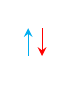
\begin{tikzpicture}
\draw[cyan,-stealth] (0,0) --++(0,10pt);
\draw[red,-stealth] (5pt,10pt) --++(0,-10pt);
\end{tikzpicture}}%
\only<3-4>{\tikz\draw[cyan,-stealth] (0,0) --++(0,10pt);}%
\only<5->{\tikz\draw[cyan,-stealth] (0,0) arc(0:360:5pt);}%
&%
\only<-2>{Circulation de l'eau}%
\only<3-4>{L'eau ne sort pas}%
\only<5->{L'eau ne rentre pas}\\
\uncover<2,4,6>{\tikz\draw[decorate,decoration={snake,segment length=4pt,amplitude=1pt,post length=2pt},-stealth,red] (0,0) --++(0,10pt);} & \uncover<2,4,6>{Conduction} \\
\uncover<2,4,6>{\tikz\draw[yellow,-stealth] (0,0) --++(0,10pt);} & \uncover<2,4,6>{Ventilation} \\
\end{tabular}}
\end{column}
\end{columns}
\end{column}
\end{columns}
\end{frame}

\begin{frame}{Combinaison}{Entretien}
\begin{block}{Après utilisation}
Bien rincer à l'eau claire, éviter l'exposition directe
au soleil.
\end{block}
\begin{block}{Longue durée}
Suspendue sur un cintre, dans un endroit sec et protégé
du soleil.

Ne pas plier et ranger dans un tiroir!
\end{block}
\end{frame}

\begin{frame}{Compléments}
\begin{itemize}
\item Cagoule (intégrée ou non);
\item gants;
\item souris;
\item chaussons, botillons\dots
\end{itemize}
\end{frame}

\subsubsection{Palmes/masque[/tuba]}

\begin{frame}{Palmes}
\centering\only<-3>{%
\begin{tikzpicture}
\node (p) at (0,0) {\includegraphics[width=10cm]{palme}};
\path (p) ++(3:2cm) coordinate (a);
\path (p) ++(64:36mm) coordinate (b);
\path (p) ++(118:16mm) coordinate (c);
\path (p) ++(23:51mm)  coordinate (d);
\path (p) ++(3:10mm) coordinate (e);
\path (p) ++(80:30mm) coordinate (f);
\draw<2>[red,stealth-stealth] (a) -- (b);
\draw<2>[red,stealth-stealth] (c) -- (d);
\node<2>[above,red] at (p.south) {Voilure};
\draw<3>[red,very thick] (e) -- (f);
\node<3>[above,red] at (p.south) {Articulation};
\end{tikzpicture}}%
\begin{block}<only@4>{Description technique}%
\begin{center}
\begin{tabular}{ll}\toprule
Voilure      & puissance disponible \\
Articulation & type de palmage*\\\bottomrule
\end{tabular}
\end{center}
\begin{minipage}{5pt}
*
\end{minipage}%
\begin{minipage}{4cm}
\begin{itemize}
\item Académique,
\item \og du genou\fg
\end{itemize}
\end{minipage}
\end{block}%
\end{frame}

\begin{frame}{Chaussantes v/s réglables}
\centering
\only<1>{\begin{tabular}{m{3cm}m{5.1cm}}
\includegraphics[height=3cm]{chaussons}                   & \includegraphics[width=5cm]{palme} \\
\includegraphics[height=3cm,angle=90,origin=c]{botillons} & \includegraphics[angle=-90,width=5cm,origin=c]{palmes_bot}\\
\end{tabular}}%
\only<2>{%
\begin{tabular}{lp{6cm}}\toprule
Chaussantes & plus petites, moins technique, plus facile, moins puissantes\\
Réglables   & plus grandes, cheville tenue, palmage en surface plus compliqué\\\midrule
\multicolumn{2}{l}{Des exceptions existent (palmes de chasse,\dots)}\\\bottomrule
\end{tabular}
}%
\end{frame}

\begin{frame}{Le masque}
\centering
\begin{block}<only@1>{}
Composé d'une jupe, du ou des verres. Doit tenir
par effet ventouse, tête en bas, plaqué par simple
inspiration.
\end{block}\only<2>{%
\begin{tikzpicture}[overlay, remember picture,pin lines/.style={help lines,thick}]
\node (pic) at (current page.center) {\includegraphics[width=\textwidth]{masques}};
\node (jupe) at (pic.north) {Jupe};
\draw[pin lines] (-3,0.5) -- (jupe);
\draw[pin lines] (2.5,0.75) -- (jupe);
\node (verre) at (pic.south) {Verres};
\draw[pin lines] (2.5,0) -- (verre);
\draw[pin lines] (-1.5,-0.5) -- (verre);
\draw[pin lines] (-4.5,-0.5) -- (verre);
\end{tikzpicture}
}
\end{frame}

\begin{frame}{Tubas}
\centering
\includegraphics[width=7cm]{tubas}
\end{frame}

\subsubsection{Petit matos}

\begin{frame}{Parachute, compas, phare, \dots}
\begin{itemize}[<+->]
\item Gants et chaussons: humides ou étanches, avec plus ou moins d'épaisseur
  de néoprène;
\item plombs: classiques, \og écologiques\fg\ ou en sac (billes);
\item couteau: classique ou plus élaboré, petit ou grand;
\item phare (lampe): pile ou batterie, puissance, encombrement, durée de fonctionnement;
\item tables de plongée: tables MN90;
\item profondimètre (ou ordinateur): fixé sur le bras, le gilet, relié à la
  bouteille, plus ou moins gros et précis;
\item compas: fixé sur le bras, le gilet, plus ou moins gros et précis;
\item parachute: plus ou moins gros, reliée à un filin souple d'une longueur
  d'environ \numprint[m]{7};
\item manomètre: sonde, plus ou moins gros et précis.
\end{itemize}
\end{frame}
